%----------------------------------------------------------------------------------------
%	PACKAGES AND DOCUMENT CONFIGURATIONS
%----------------------------------------------------------------------------------------
\documentclass[article, a4paper, 11pt, oneside]{memoir}

% Margins
\usepackage[top=3cm,left=2cm,right=2cm,bottom=3cm]{geometry}

% Encondings
\usepackage[utf8]{inputenc}

% Language
\usepackage[portuguese]{babel}

% Graphics and images
\usepackage{graphicx}
	\graphicspath{{./images/}}

% Listings
\usepackage{listings}
\lstset{language=C}
\usepackage{color}
\definecolor{dkgreen}{rgb}{0,0.6,0}
\definecolor{gray}{rgb}{0.5,0.5,0.5}
\definecolor{mauve}{rgb}{0.58,0,0.82} 

\lstset{frame=tb,
  language=C,
  aboveskip=3mm,
  belowskip=3mm,
  showstringspaces=false,
  columns=flexible,
  basicstyle={\small\ttfamily},
  numbers=none,
  numberstyle=\tiny\color{gray},
  keywordstyle=\color{blue},
  commentstyle=\color{dkgreen},
  stringstyle=\color{mauve},
  breaklines=true,
  breakatwhitespace=true,
  tabsize=3
}

\usepackage{amsmath}

% Color
\usepackage[dvipsnames]{xcolor}

% Tables
\usepackage{tabularx}

% Math symbols
\usepackage{amssymb}

% Paragraph Spacing
\usepackage{parskip}
\usepackage{indentfirst}
\setlength{\parskip}{0.2cm}

% Hyperreferences
\usepackage{hyperref}

% Repeated commands
\usepackage{expl3}
\ExplSyntaxOn
\cs_new_eq:NN \Repeat \prg_replicate:nn
\ExplSyntaxOff

% Header and Footer Things
\usepackage{wallpaper}
\usepackage{fancyhdr}

% Following code to edit the pagestyle
\pagestyle{fancy}
\fancyhf{}
\rhead{RCOM}
\lhead{Redes de Computadores}
\rfoot{Página \thepage}

% Commands
\usepackage{xargs}

%% Linked Email
\newcommand{\email}[1]{
{\texttt{\href{mailto:#1}{#1}} }
}

%----------------------------------------------------------------------------------------
%	DOCUMENT INFORMATION
%----------------------------------------------------------------------------------------
% Title
\title{\Huge \texttt{Redes de Computadores} }
% Authors
\author{
\LARGE \textbf{Turma 1 Grupo 5}\\\\
\begin{tabular}{l r}
	  Diogo Samuel Gonçalves Fernandes	& \email{up201806250@fe.up.pt}\\
	 Paulo Jorge Salgado Marinho Ribeiro  & \email{up201806505@fe.up.pt}\\
\end{tabular}
}

% Date for the report
\date{\today}

% Table of Contents
\addto\captionsportuguese{\renewcommand*\contentsname{Índice}}

%----------------------------------------------------------------------------------------
%	DOCUMENT
%----------------------------------------------------------------------------------------
\begin{document}
%----------------------------------------------------------------------------------------
%	Front Page
%----------------------------------------------------------------------------------------
% Title Author and Date
\maketitle

+% More information for front page
\begin{center}
\textbf{Projeto RCOM - 2019/20 - MIEIC}
\Repeat{2}{\linebreak}
\begin{tabular}{l r}
	\textbf{Professor}: 
	\begin{tabular}{l r}
		Rui Campos & \email{rcampos@fe.up.pt}	\\
	\end{tabular}
\end{tabular}
\Repeat{4}{\linebreak}

\end{center}

\newpage
%----------------------------------------------------------------------------------------
%	CHAPTER 1 - Descrição do Problema
%----------------------------------------------------------------------------------------
\chapter[Introdução][Introdução]{Introdução} \label{\thechapter}

Este trabalho consiste no desenvolvimento de uma aplicação de download via ftp e na criação de uma rede. O trabalho está portanto, dividido em duas partes distintas:

- Parte 1 - Aplicação de download
- Parte 2 - Configuração de uma rede

%----------------------------------------------------------------------------------------
%	CHAPTER 2 - Parte 1 - Aplicação de download
%----------------------------------------------------------------------------------------
\chapter[Aplicacao][Aplicacao]{Aplicacao} \label{\thechapter}

A primeira parte deste segundo projeto consiste no desenvolvimento de uma aplicação de download,
que permite transferir um ficheiro de qualquer tipo, de um dado servidor FTP. Após compilar o código
recorrendo ao comando "make", o utilizador deve escrever na consola o seguinte comando, para correr o programa:

./download ftp://[user]:[pass]@[host]/[url-path]

O campo [user] deverá conter o username com que o utilizador deseja entrar no servidor, e [pass] a respetiva password.
No caso de desejar entrar de forma anónima, o utilizador deverá introduzir o username "anonymous" e uma qualquer password.
O campo [host] indicará o endereço do servidor FTP ao qual se deseja conectar, e [url-path] o caminho para o ficheiro que se pretende transferir.

- Arquitetura

A estrutura principal do programa encontra-se bem explícita no ficheiro clientTCP.c.
O programa começa por processar o argumento introduzido pelo utilizador, armazenando o seu username,
pass, o host, e o path para o ficheiro, recorrendo à função parseArguments(), definida no ficheiro utils.c. 
Se o input recebido for inválido, o programa termina e é apresentada uma mensagem indicando a correta utilização do programa.

De seguida, é processado o campo host, obtendo-se o correspondente IP Adress, com recurso à função getIP().
Este IP Adress é utilizado logo a seguir, na conexão ao servidor, após criação de um socket que será utilizado
para troca de comandos entre o cliente e o servidor.

Após conectar este socket ao servidor desejado, é lida a resposta do servidor, a qual se espera que contenha o código 220,
que indica que a conexão foi estabelecida e que o servidor espera pelo login de um novo utilizador. 

Assim, o próximo passo será efetuar o login (função login()), que consiste numa troca de mensagens entre o cliente e o servidor,
estabelecida da seguinte forma:

  - Envio do comando "user [user] newline", em que [user] é o username recebido como input
  - Receção da resposta ao comando user. Se o primeiro dígito do código recebido for 2, então não é requerida password, e o login é efetuado com sucesso. Se esse dígito for 3, então é necessária uma password, e os próximos passos são efetuados.
  - Envio do comando "pass [pass] newline", em que [pass] é a password recebida como input
  - Receção da resposta ao comando pass. Se o código recebido for 230, então a password foi aceite e o login foi efetuado com sucesso. Caso contrário, o programa termina acusando erro no login.

Após sucesso no login, é necessário pedir ao servidor para transferir dados em modo passivo. Isto é efetuado na função activatePassiveMode(), que começa por enviar o comando "pasv newline" para o servidor.
Segue-se uma máquina de estados, que vai receber a resposta do servidor a este comando, e que vai armazenar os valores retornados, utilizando-os para calcular a porta para a qual serão enviados os dados. 

Após isto, é efetuada a criação de um novo socket e a sua conexão ao servidor, pela porta resultante do passo anterior, de onde serão lidos os dados do ficheiro.

Já com tudo configurado, é efetuada a transferência do ficheiro, na função download\textunderscore file(), que começa por mandar
o comando "retr [path] newline" para pedir o ficheiro desejado. Segue-se a leitura da resposta do servidor face a este comando,
a qual se espera ser o código 150, que indica que o ficheiro está pronto para download e o pedido foi aceite. 
Assim, pode-se começar a ler a informação do ficheiro, do socket aberto para leitura dos dados, e enviar a informação para um ficheiro criado imediatamente antes,
cujo nome é obtido aplicando a função basename() ao path recebido como input. Se não tiver ocorrido nenhum erro durante o processo, é apresentada uma mensagem de sucesso,
que indica que o ficheiro foi transferido. 

Por último, o programa fecha os dois sockets abertos.

- Resultados

O nosso programa foi testado para diversos casos, nomeadamente a utilização de diferentes servidores FTP,
diferentes logins (introdução de username e password e entrada em modo anónimo), e utilização de diferentes tipos e tamanhos, nos ficheiros transferidos.
Para maior compreensão do processo, são imprimidos na consola todos os passos efetuados, assim como as respetivas respostas do servidor.
Concluímos todos os requisitos desta primeira parte com sucesso, pelo que a aplicação encontra-se totalmente funcional.

%----------------------------------------------------------------------------------------
%	CHAPTER 3 - Parte 2 - Experiencias de rede
%----------------------------------------------------------------------------------------
\chapter[Rede][Rede]{Rede} \label{\thechapter}

\section{Experiência 1 - Configurar uma rede IP}

Nesta primeira experiência foi ligado o \emph{gnu63} ao \emph{gnu64}, recorrendo à configuração dos seus endereços IP para que pudessem comunicar entre si. 
COLOCAR COMANDOS IFCONFIG AQUI
Esta conexão foi testada recorrendo ao comando ping.

O ARP (Address Resolution Protocol) é um protocolo utilizado para obter o endereço MAC associado
a um dado endereço de IP. Para o envio de uma trama para um dado computador presente na rede, o emissor
necessita do endereço MAC correspondente ao endereço IP de destino. Para isto, é enviado um pacote ARP
em modo Broadcast, que contém esse IP e que espera o retorno do endereço MAC desejado.
Isto pode ser observado na Figura 1, no pacote número 23 em que é enviado um pacote ARP em broadcast.

Após fazermos ping do gnu63 para o gnu64, para além dos pacotes ARP são gerados pacotes ICMP(Internet Control Message Protocol), 
o que pode ser observado na \emph{Figura 1}.
É também possível verificar que os IPs de origem e destino dos pacotes ping são os IPs e MACs do gnu63 e do gnu64, respetivamente.
A distinção entre tramas Ethernet do tipo ARP, IP ou ICMP pode ser feita analisando o cabeçalho dessa trama, que terá valores distintos conforme o tipo de trama.
Por sua vez, o comprimento das tramas pode ser obtido no wireshark, como consta na figura ?, uma vez que essa informação está também presente no cabeçalho da trama.

A interface loopback é responsável por realizar o diagnóstico de problemas e testes de conectividade.
É o método mais usado para determinar se um dispositivo está online, e está presente na figura ?.


\section{Experiência 2 - Implementar duas LAN virtuais num switch}

Nesta experiência, foram criadas duas LANs virtuais, estando os computadores gnu63 e gnu64 conectados à VLAN 60 e o gnu62 conectado à VLAN 61.
O gnu62 uma vez que se encontra numa rede diferente do gnu63 e gnu64 não consegue comunicar com os mesmos.

Para criar as VLANs, tivemos de configurar o switch adicionando-as usando o comando vlan <yN>, 
em que y era o número da bancada e N o número que identifica a vlan. Seguiu-se a configuração das vlans,
onde foi necessário adicionar as portas do switch às respetivas VLANs, recorrendo aos comandos 
<interface fastethernet 0/n> em que n é a porta do switch, <switchport mode access> e <switchport access vlan yN>.

Após este processo, passam a existir dois domínios de transmissão, sendo que um contém o gnu63 e gnu64 e o outro contém gnu62.

Deste modo, quando é feito ping em modo de broadcast a partir do gnu63, o gnu64 como se encontra na mesma VLAN irá conseguir 
receber esses pacotes como é possível constatar com as figuras 4 e 5, enquanto que o gnu62 não recebe qualquer pactoe uma vez que se encontra noutra VLAN.
Da mesma forma, quando é feito ping em modo de broadcast a partir do gnu62, quer o gnu63 quer o gnu64 não irão receber qualquer pacote, como se pode verificar
nas figuras 7 e 8, uma vez que estes dois se encontram numa rede diferente.


\section{Experiência 3 - Configurar Router em Linux}

Nesta experiência, o gnu64 foi configurado de modo a funcionar como um router, estabelecendo assim a ligação entre as duas VLANs criadas anteriormente.

Para isto, configurou-se a porta eth1 do gnu64 com um IP no mesmo domínio que o gnu62. Depois, foi necessário configurar as rotas com o comando <route add>. No gnu63 adicionou-se a rota
que redireciona os pacotes para o endereço IP do gnu64 relativo à segunda vlan, e o mesmo foi realizado para o gnu62, mas com o IP relativo à primeira vlan.
Tudo isto pode ser verificado na figura ?.
Após isto, torna-se possível realizar ping do gun63 para o gun62, uma vez que os pedidos são encaminhados para o gnu64, que consegue comunicar com os outros dois PCs.

A tabela de forwarding define a forma como uma trama será encaminhada de um switch ou router na rede. Contém o destino da rota, a "gateway", que corresponde ao próximo ponto por onde a rota passará,
a máscara (netmask), usada para determinar o ID da rede a partir do endereço IP de destino, informações e custo da rota, o número de referências para a rota, um contador de pesquisas da rota, e a placa de rede responsável pela gateway.

Sempre que um dos PCs dá ping a outro e o PC que recebeu o pedido não conhece o endereço MAC do emissor, envia um pacote ARP a pedir esta informação, como mostrado na experiência 1, que conterá os endereços dos PCs de origem e de destino.
Os pacotes ICMP observados resultam do comando ping, e tratam-se de pacotes de request e reply, uma vez que ,após a configuração desta experiência, todos os PCs conseguem comunicar entre si.
No caso de não conseguirem comunicar entre si, seriam enviados pacotes ICMP do tipo Host Unreachable.
Os endereços IP e MAC dos pacotes ICMP são os dos PCs de origem e destino.

figura ? - meter figuras

\section{Experiência 4 - Configurar um Router comercial e implementar NAT}

Nesta experiência, configuramos o router do laboratório, ligando-o à rede local. Posteriormente, configuramos este router
com NAT, de modo a que todos os computadores da rede tivessem acesso à Internet. Neste caso, apenas o gnu64 não terá acesso à Internet, por não se encontrar na lista de IPs acessíveis do router.

// figura ? - EXPLICAR PERGUNTA 1

Os pacotes enviados durante esta experiência seguem uma dada rota, no caso de esta já estar definida. Caso contrário, estes são direcionados para a rota default do router,
que indica que o gnu64 existe, e portanto os pacotes serão enviados para este.

Posteriormente, configurou-se NAT no router, usando os comandos presentes no slide 46 do guião deste projeto, que começam por configurar as duas interfaces do router.
O NAT (Network Address Translation) tem como objetivo poupar espaço de endereçamento público, dado que os IPs públicos são limitados e escassos.
Resumidamente, permite que as redes privadas que usam endereços IPs não registados se conetem à Internet ou a uma rede pública, ao traduzir estes endereços em endereços legais. 
Desta forma, apenas um endereço IP é exigido, que irá representar todos os computadores da rede local.

\section{Experiência 5 - DNS}			

Nesta experiência, foi configurado o DNS (Domain Name Service). Trata-se de um sistema hierárquico e distribuído de gestão de nomes para computadores, serviços ou qualquer máquina conectada à Internet ou a uma rede privada.
Isto é, é um sistema que traduz os hostnames nos respetivos endereços IP, recorrendo a servidores de DNS que contém uma base de dados com esta correspondência entre hostnames e IPs.

Para a sua configuração foi necessário alterar o ficheiro resolv.conf, adicionando o nome do servidor de DNS e o seu endereço IP, de acordo com o slide 14 do guião do projeto.

Quando se faz ping a um servidor externo, é enviado um pacote de DNS com o pedido do IP do servidor. A resposta chega na forma de um outro pacote DNS, que após fazer a conversão, devolverá o endereço IP correspondente.
Esta troca de pacotes pode ser observada na figura ?

\section{Experiência 6 - TCP connections}

Esta experiência serviu para observação do comportamento do protocolo TCP, 
recorrendo à aplicação que desenvolvemos na parte 1 deste projeto. 

A aplicação estabelece duas conexões TCP - uma para troca de comandos entre o cliente e o servidor FTP, que trata do transporte do controlo de informação FTP, e outra para a receção dos dados enviados pelo servidor.
Cada conexão FTP subdivide-se em três fases: o estabelecimento da conexão, a troca de dados entre o cliente e servidor, e o encerramento da conexão.
O mecanismo ARQ (Automatic Repeat Request) do TCP (Transmission Control Protocol) é utilizado com o método da janela deslizante, e consiste no controlo dos erros que ocorram durante a transmissão dos dados.
Recorre a "acknowledgement numbers", que estão incluídos nas tramas enviadas pelo recetor, indicando se esta foi recebida corretamente, sem quaisquer problemas, e recorre também ao "window size", que indica o domínio de pacotes possíveis de ser enviados pelo emissor, e ao "sequence number", que indica o número do pacote a ser enviado.
O TCP usa um mecanismo de controlo de congestão end-to-end. Isto significa que o emissor limita ou aumenta a taxa de entrega de dados para conexão em função do congestionamento percebido por ele.
A conexão TCP é composta por diversas variáveis, sendo uma delas a janela de congestionamento, que limitará a taxa de envio de pacotes de um dado emissor TCP.
Os gráficos obtidos durante a experiência (figura ?) permitem concluir que no início do primeiro download no gnu63, a taxa de transferência aumentou, e após o segundo download verificou-se uma rápida descida seguida de uma ligeira subida, que estabilizou num nível mais baixo do que o nível inicial.
Assim, conclui-se que o fluxo dos dados está de acordo com o mecanismo de controlo de congestão, tendo em conta que se observa um menor bitrate no momento em que a rede estava mais congestionada (mais downloads simultâneos).

Com o aparecimento de uma segunda conexão TCP, dá-se uma diminuição da taxa de transferência, tendo em conta que esta é distribuída igualmente para cada ligação.

%----------------------------------------------------------------------------------------
%	CHAPTER 4 - Conclusões
%----------------------------------------------------------------------------------------
\chapter[Conclusões][Conclusões]{Conclusões} \label{\thechapter}

Este segundo projeto da unidade curricular Redes de Computadores teve como objetivo, numa primeira parte, a implementação de uma aplicação de download de ficheiros recorrendo ao protocolo FTP,
e, numa segunda parte, à configuração de uma rede de computadores. Apesar de dificultado pelo reduzido tempo que tivemos para aproveitar o laboratório, devido à situação pandémica que atualmente enfrentamos,
este projeto foi terminado com sucesso, sendo que conseguimos desenvolver todos os aspetos pedidos.
Ao mesmo tempo, interiorizamos conceitos importantes nesta área, e compreendemos os diversos protocolos que foram abordados.

Em suma, conseguimos alcançar todos os nossos objetivos, e conhecemos conceitos dos quais nunca antes tínhamos ouvido falar, mas que utilizavamos com frequência no nosso dia-a-dia.

\newpage
%----------------------------------------------------------------------------------------
%	CHAPTER 5 - Anexos
%----------------------------------------------------------------------------------------
\chapter[Anexos][Anexos]{Anexos} \label{\thechapter}

\section{Anexo I - Imagens}
\subsection{Experiência 1}

\begin{figure}[h]
	\centering
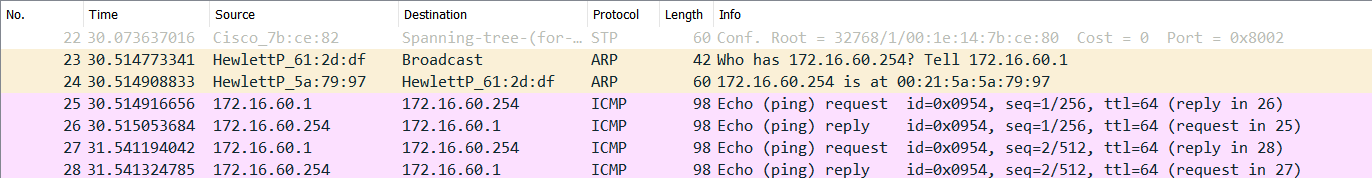
\includegraphics[scale=0.55]{exp1-gnu63.png}
\caption{Ping gnu64 from gnu63}
\end{figure}

exp2-step5-ping-gnu62-from-63

\subsection{Experiência 2}
\begin{figure}[h]
	\centering
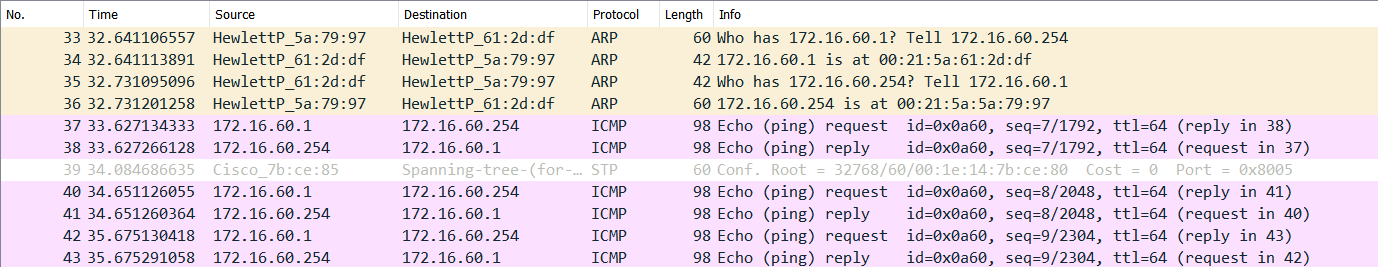
\includegraphics[scale=0.55]{exp2-step5-ping-gnu64-from-gnu63.png}
\caption{Ping gnu64 from gnu63}
\end{figure}

\newpage
\begin{figure}[h]
	\centering
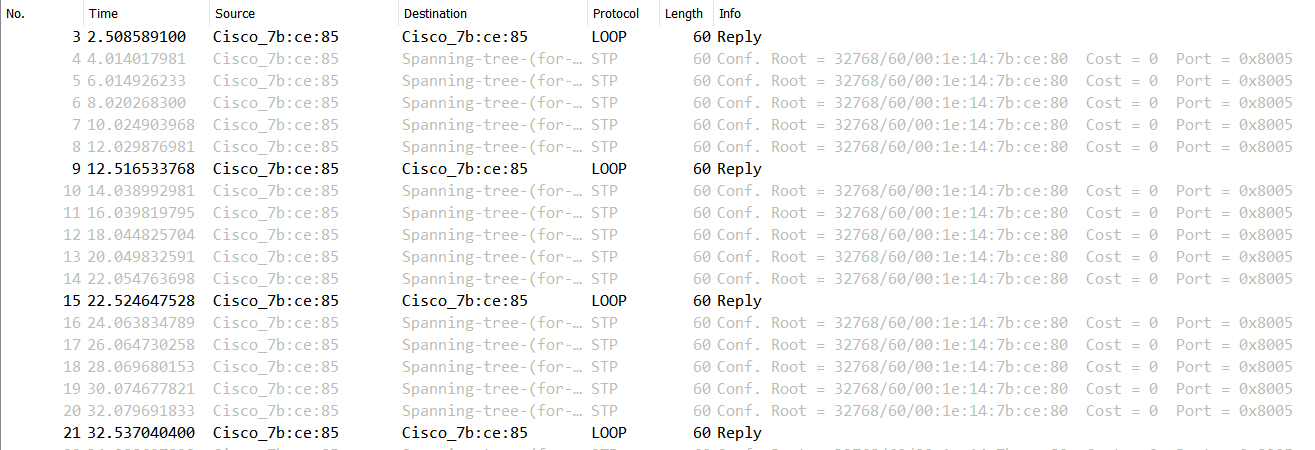
\includegraphics[scale=0.55]{exp2-step8-broadcast-gnu63-from-gnu62.png}
\caption{Ping broadcast a partir do gnu63 (ping –b 172.16.60.255) capturado no gnu62}
\end{figure}

\begin{figure}[h]
	\centering
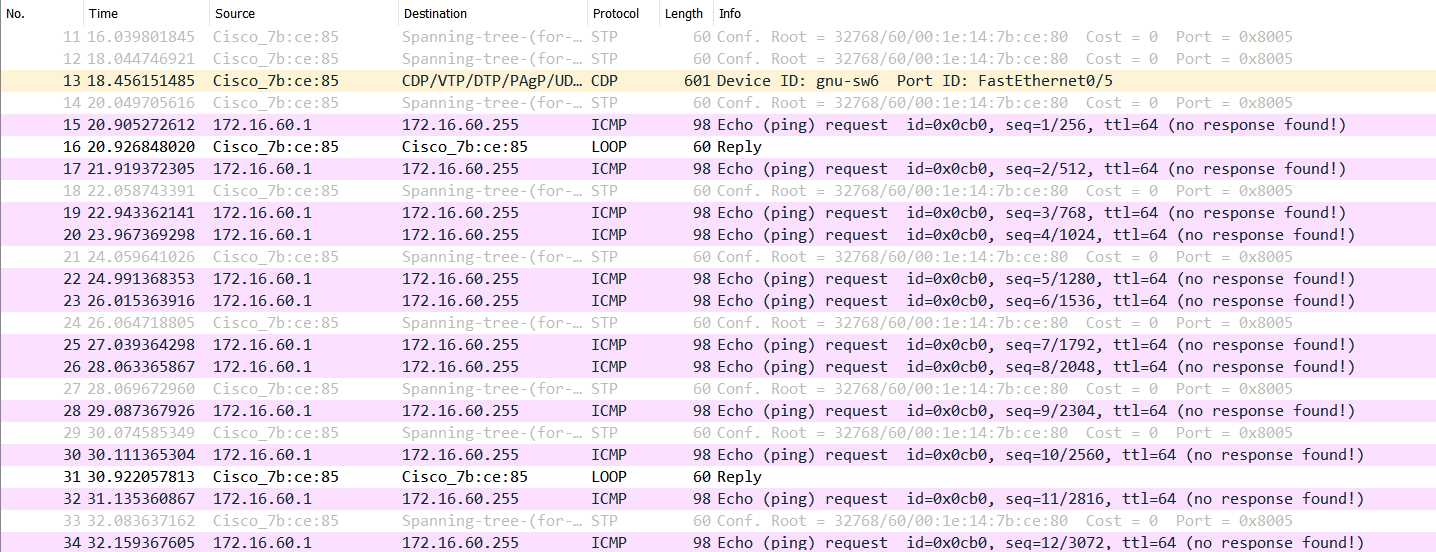
\includegraphics[scale=0.55]{exp2-step8-broadcast-gnu63-from-gnu63.png}
\caption{Ping broadcast a partir do gnu63 (ping –b 172.16.60.255) capturado no gnu63}
\end{figure}

\begin{figure}[h]
	\centering
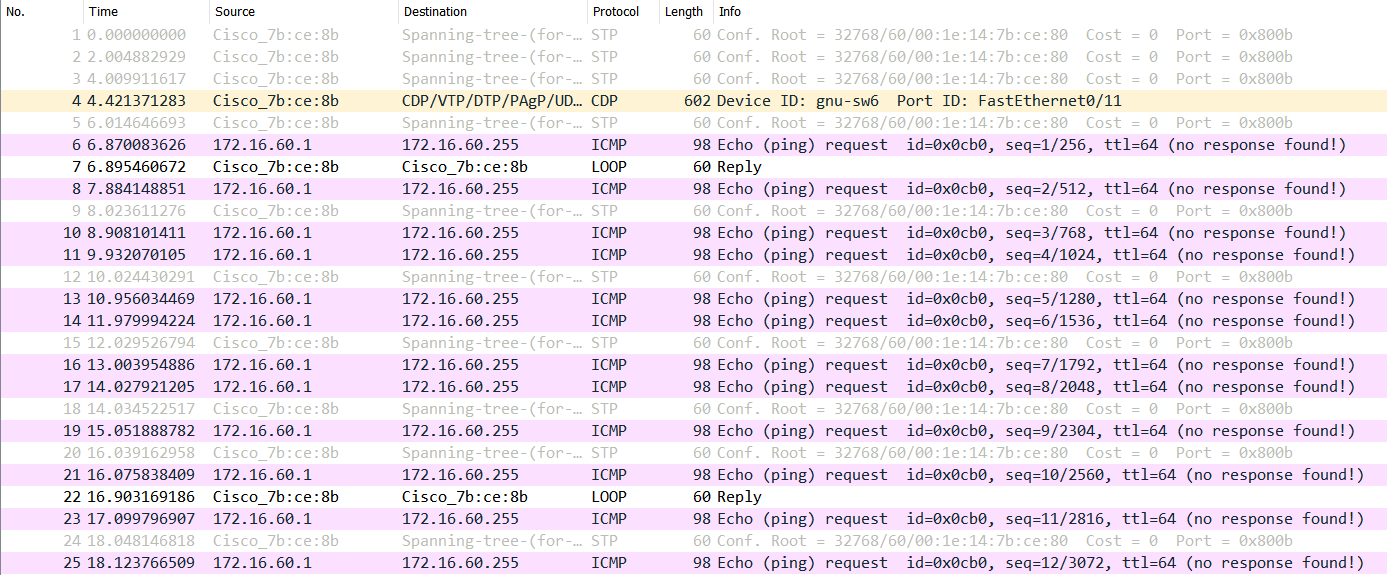
\includegraphics[scale=0.55]{exp2-step8-broadcast-gnu63-from-gnu64.png}
\caption{Ping broadcast a partir do gnu63 (ping –b 172.16.60.255) capturado no gnu64}
\end{figure}

\newpage
\begin{figure}[h]
	\centering
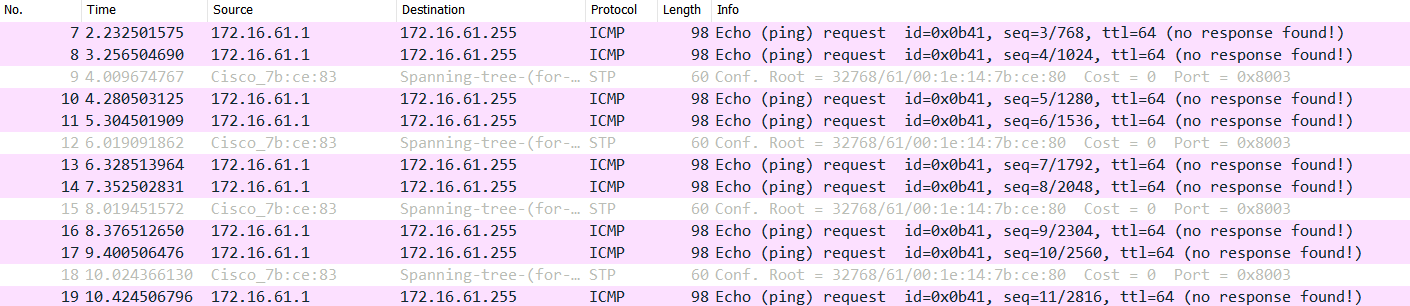
\includegraphics[scale=0.55]{exp2-step10-broadcast-gnu62-from-gnu62.png}
\caption{Ping broadcast a partir do gnu62 (ping –b 172.16.61.255) capturado no gnu62}
\end{figure}

\begin{figure}[h]
	\centering
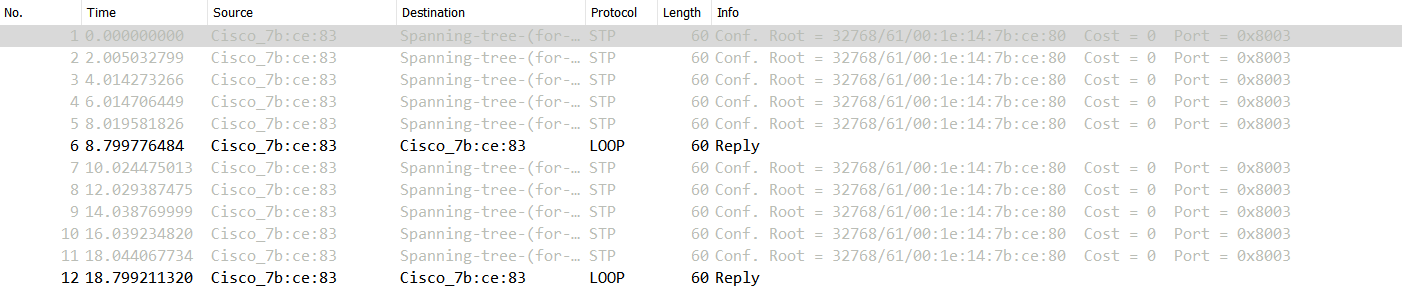
\includegraphics[scale=0.55]{exp2-step10-broadcast-gnu62-from-gnu63.png}
\caption{Ping broadcast a partir do gnu62 (ping –b 172.16.61.255) capturado no gnu63}
\end{figure}

\begin{figure}[h]
	\centering
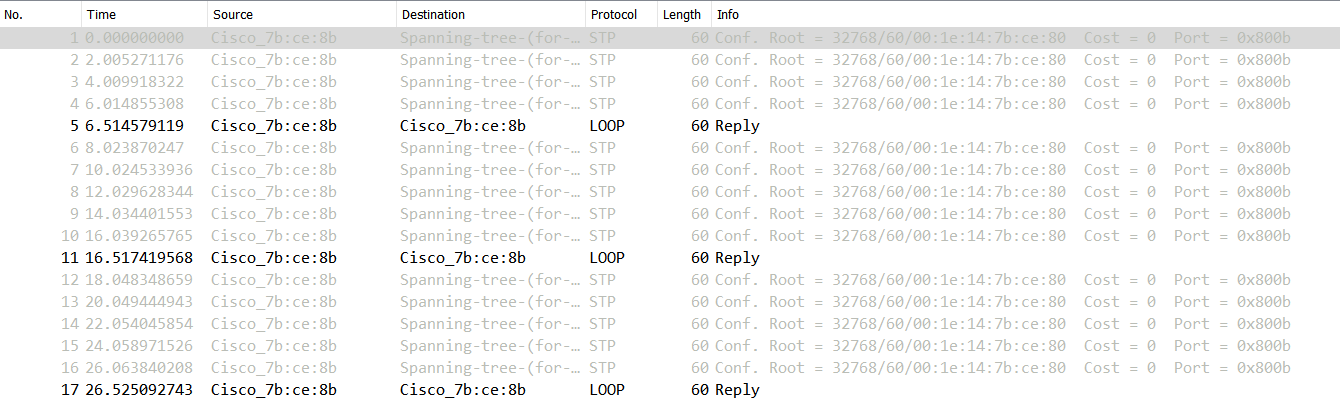
\includegraphics[scale=0.55]{exp2-step10-broadcast-gnu62-from-gnu64.png}
\caption{Ping broadcast a partir do gnu62 (ping –b 172.16.61.255) capturado no gnu64}
\end{figure}

\newpage
\subsection{Experiência 3}
\begin{figure}[h]
	\centering
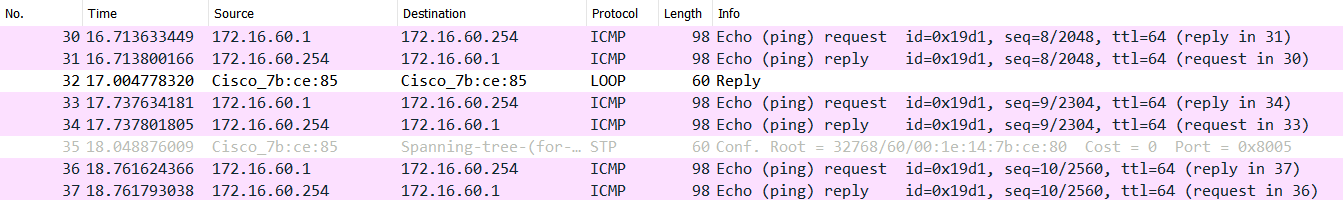
\includegraphics[scale=0.55]{exp3-step6-ping-60.254-from-gnu63.png}
\caption{Ping 172.16.60.254 a partir do gnu63}
\end{figure}

\begin{figure}[h]
	\centering
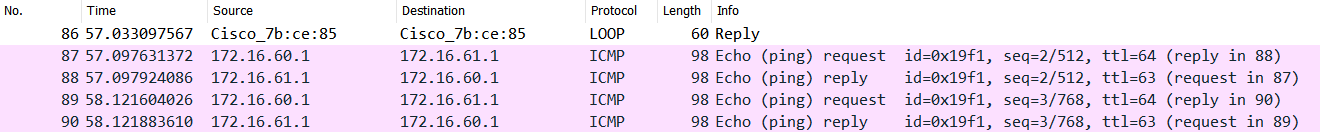
\includegraphics[scale=0.55]{exp3-step6-ping-61.1-from-gnu63.png}
\caption{Ping 172.16.61.1 a partir do gnu63}
\end{figure}

\begin{figure}[h]
	\centering
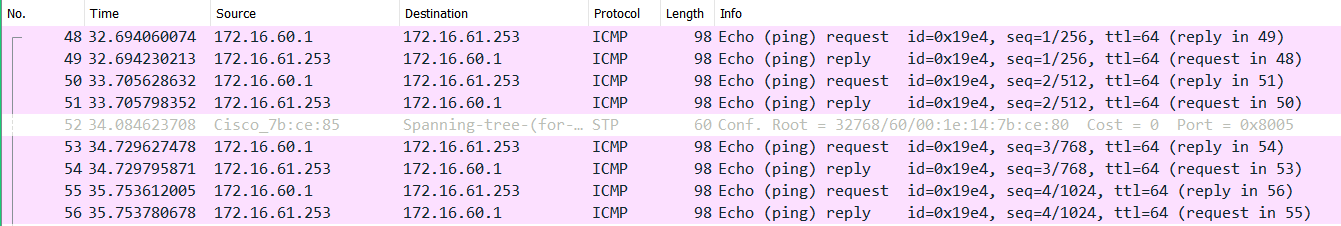
\includegraphics[scale=0.55]{exp3-step6-ping-61.253-from-gnu63.png}
\caption{Ping 172.16.61.253 a partir do gnu63}
\end{figure}

VERIFICAR STEP 10

\newpage
\begin{figure}[h]
	\centering
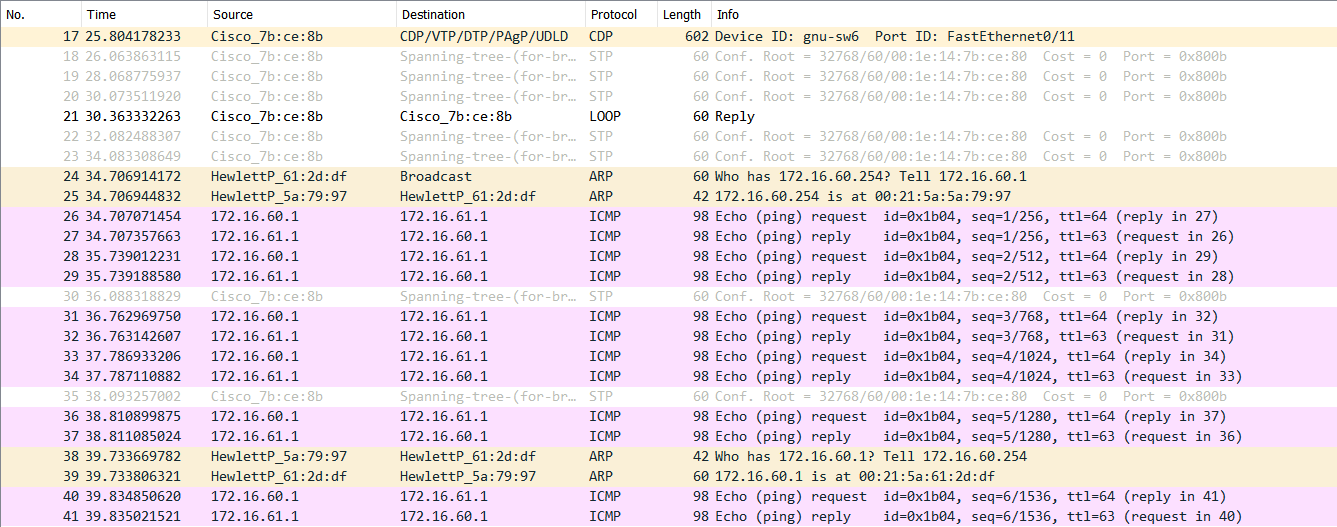
\includegraphics[scale=0.55]{exp3-step10-ping-gnu62-from-gnu63-eth0.png}
\caption{Ping do gnu62 para gnu63 e capturar no eth0 do gnu64}
\end{figure}

\begin{figure}[h]
	\centering
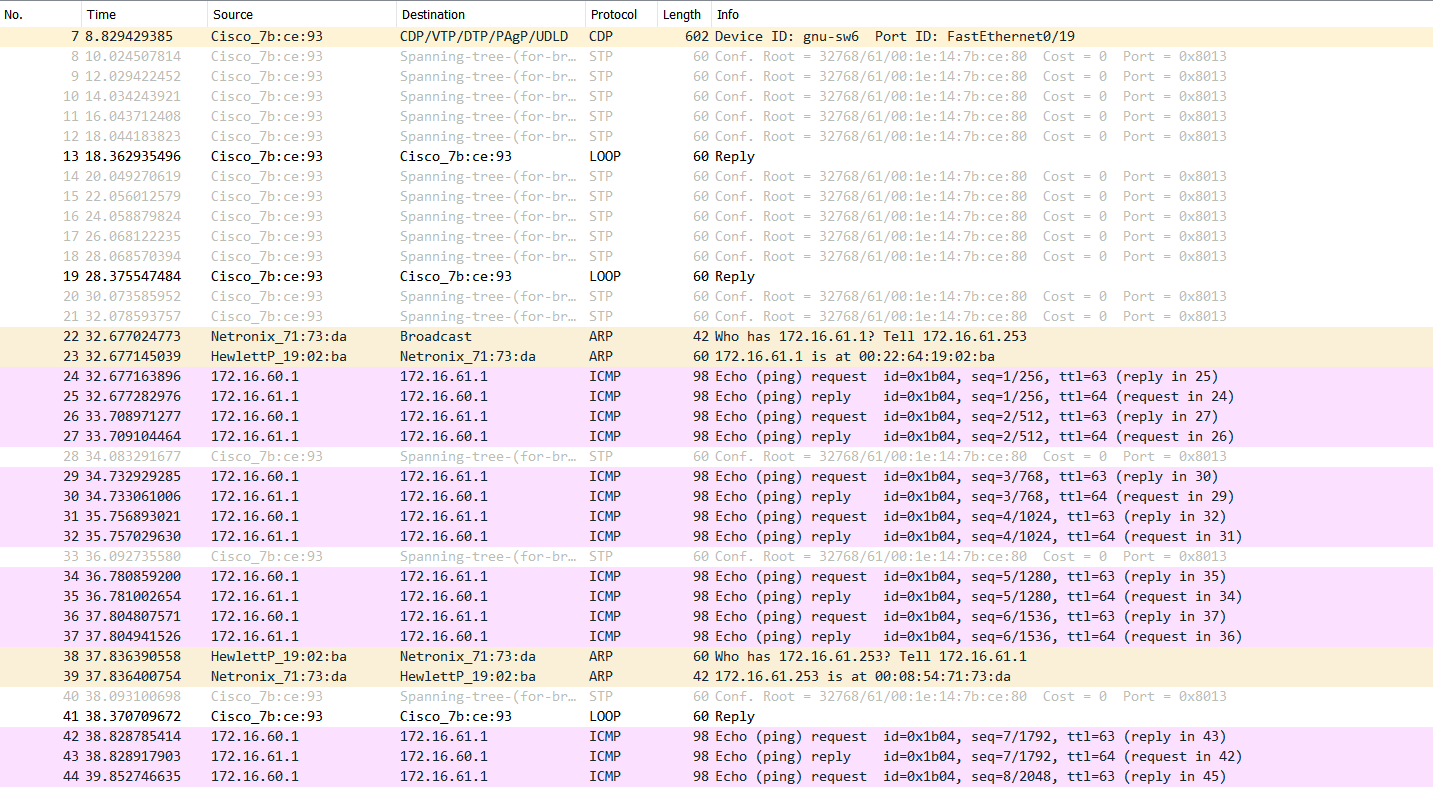
\includegraphics[scale=0.55]{exp3-step10-ping-gnu62-from-gnu63-eth1.png}
\caption{Ping do gnu62 para gnu63 e capturar no eth1 do gnu64}
\end{figure}

\subsection{Experiência 4}
FALTA A EXP 4

\newpage
\subsection{Experiência 5}
\begin{figure}[h]
	\centering
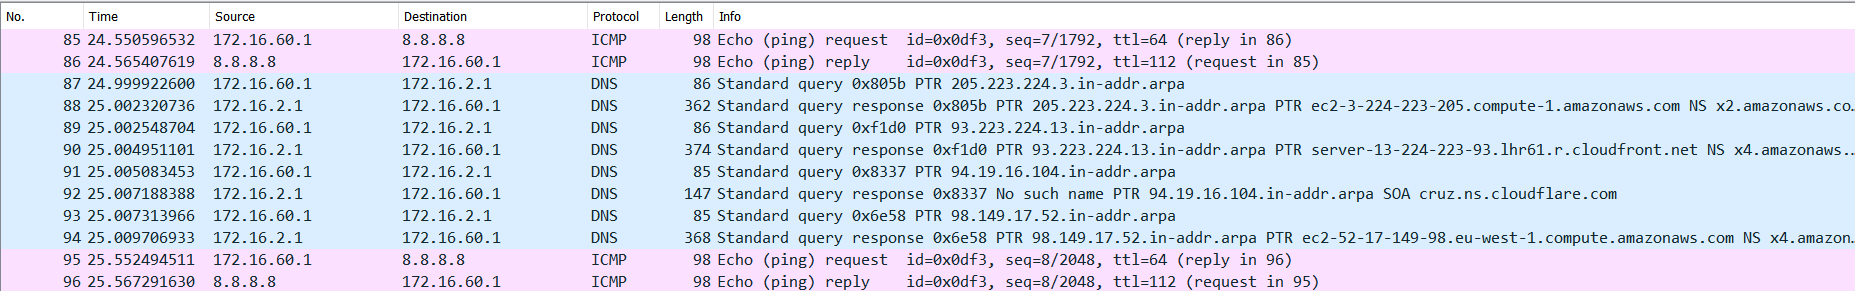
\includegraphics[scale=0.55]{exp5-step3.png}
\caption{Ping 8.8.8.8}
\end{figure}


\subsection{Experiência 6}
\begin{figure}[h]
	\centering
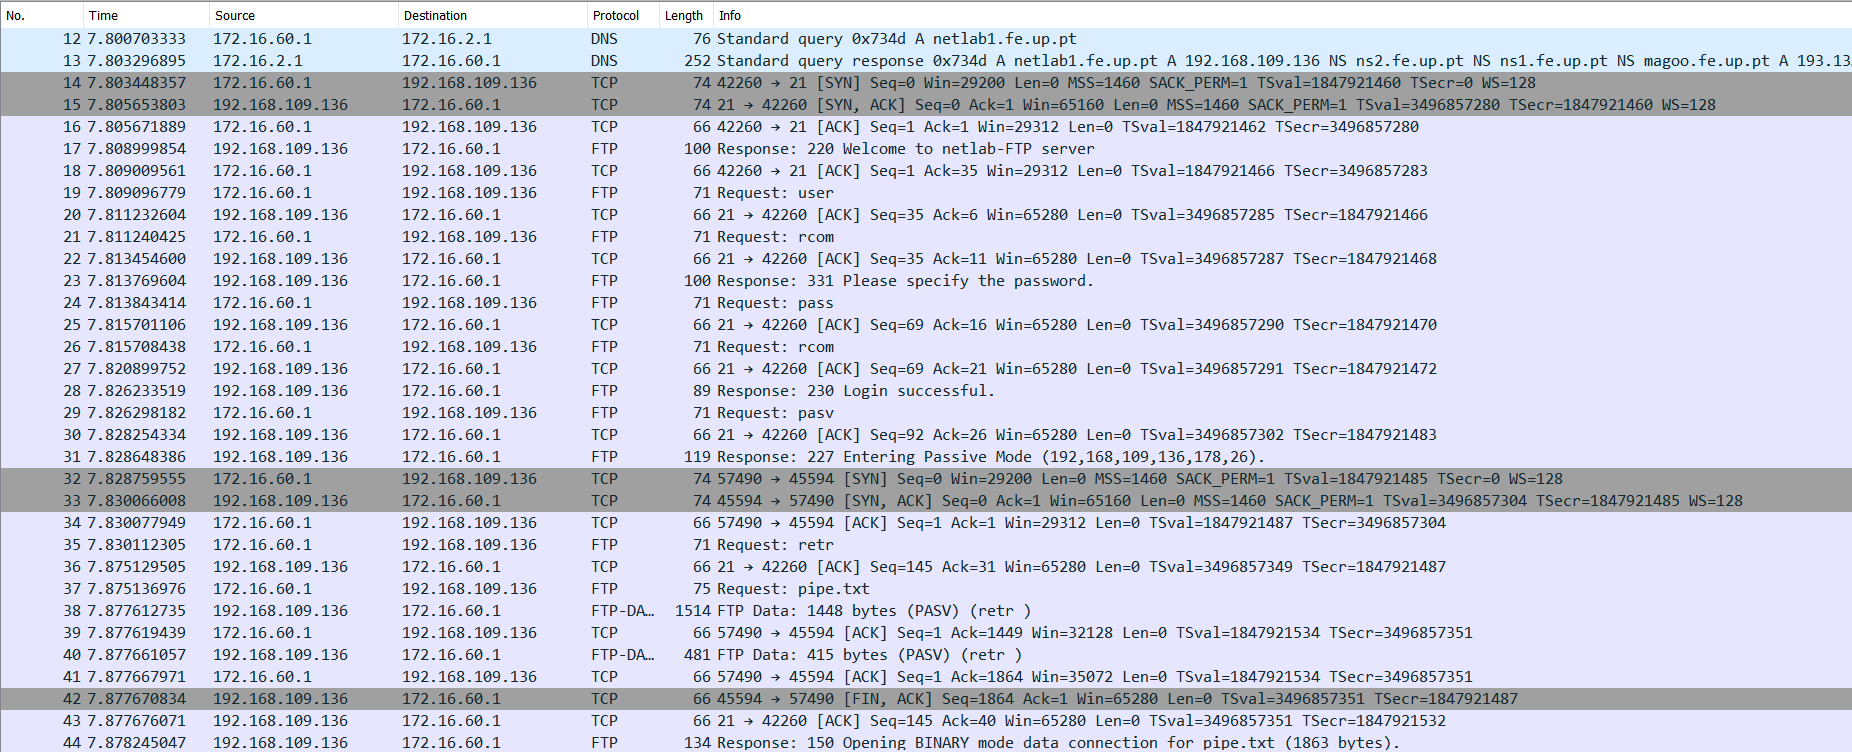
\includegraphics[scale=0.55]{exp6-step3-part1.png}
\caption{FTP download - Part 1}
\end{figure}

\begin{figure}[h]
	\centering
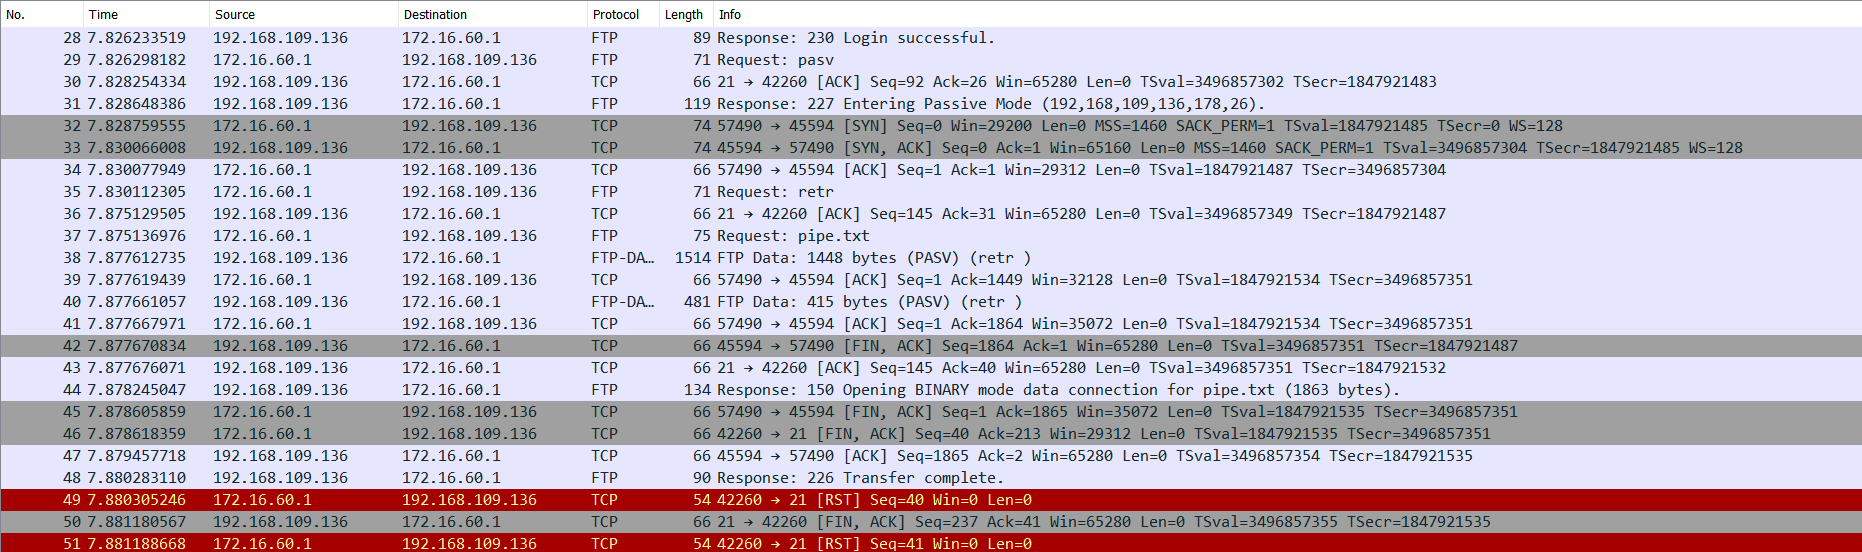
\includegraphics[scale=0.55]{exp6-step3-part2.png}
\caption{FTP download - Part 2}
\end{figure}

\newpage
\begin{figure}[h]
	\centering
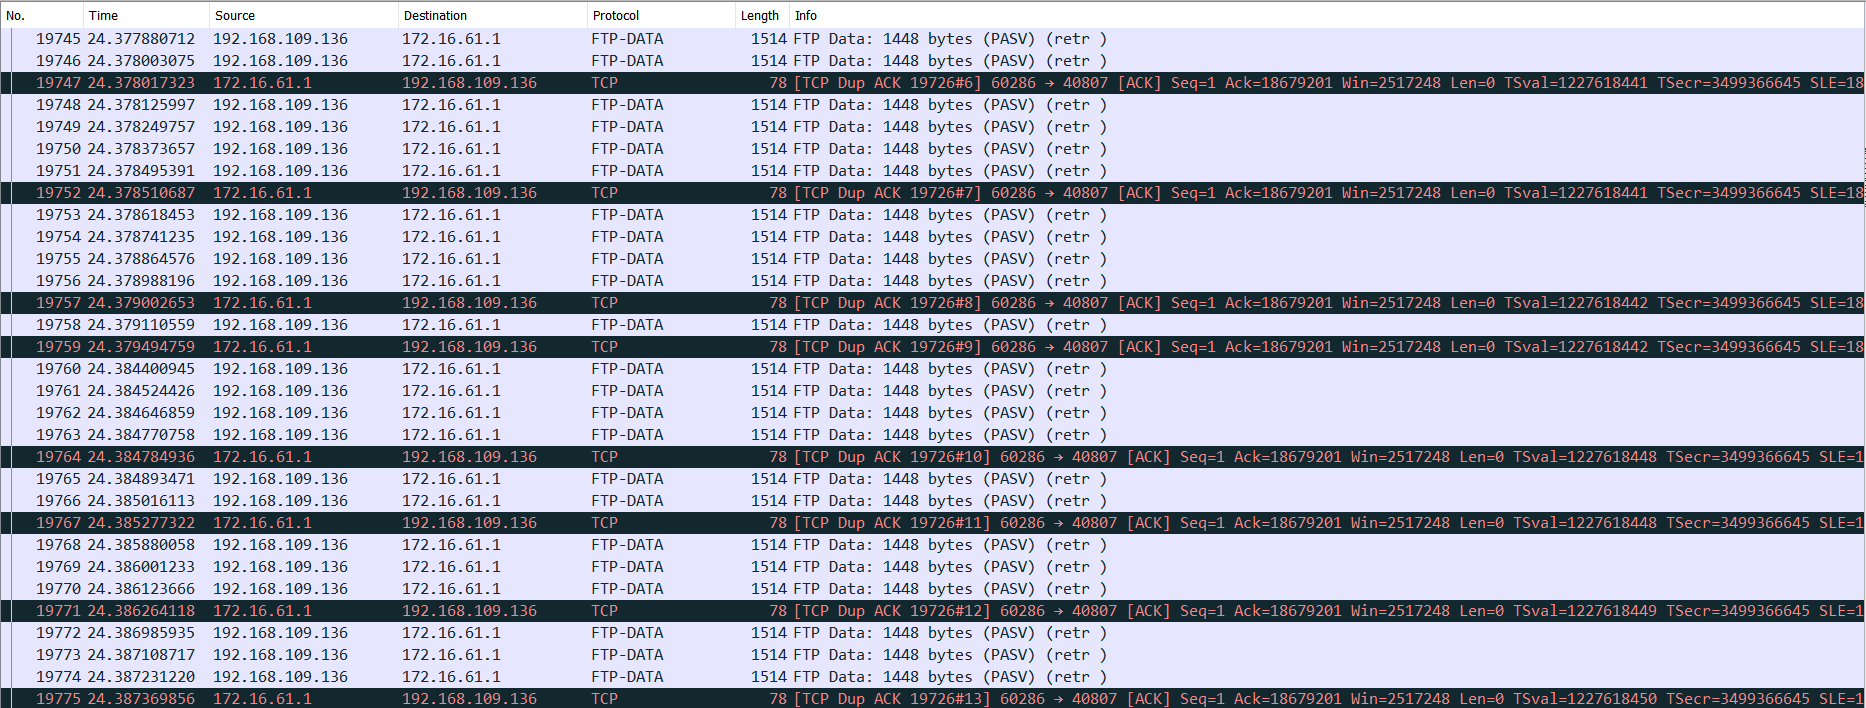
\includegraphics[scale=0.55]{exp6-step5-error.png}
\caption{DUP ACK durante a transferência}
\end{figure}

\begin{figure}[h]
	\centering
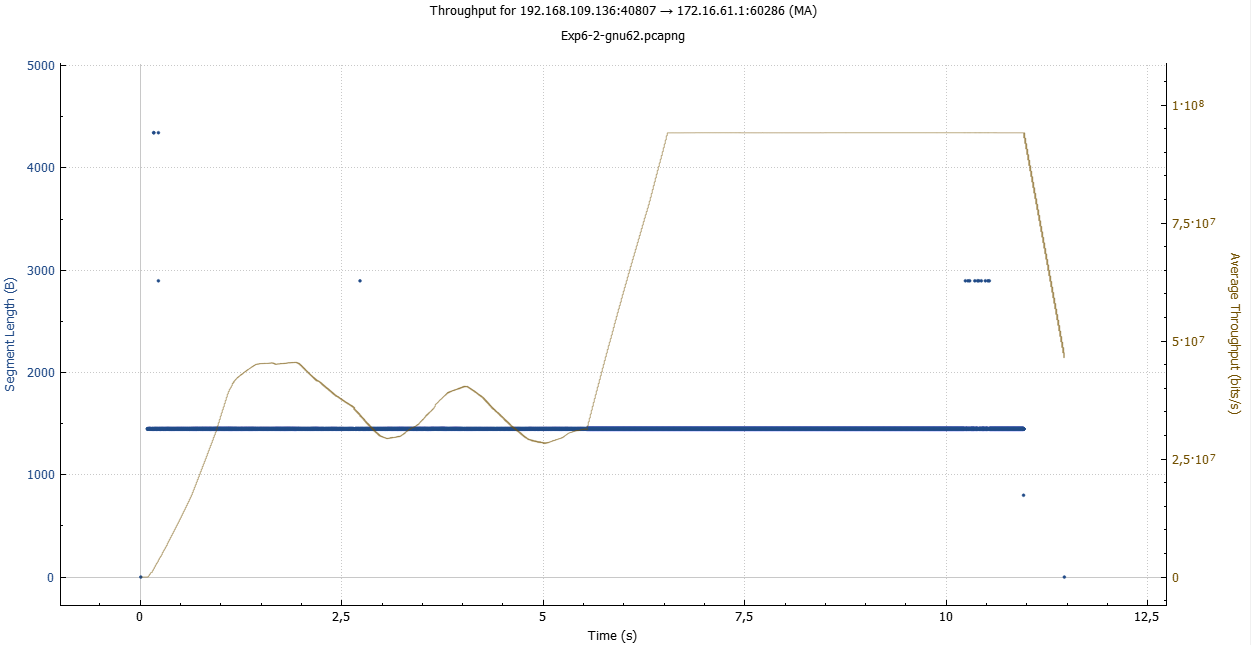
\includegraphics[scale=0.55]{exp6-step5-gnu62-graph.png}
\caption{Taxa de transferência no gnu62}
\end{figure}

\begin{figure}[h]
	\centering
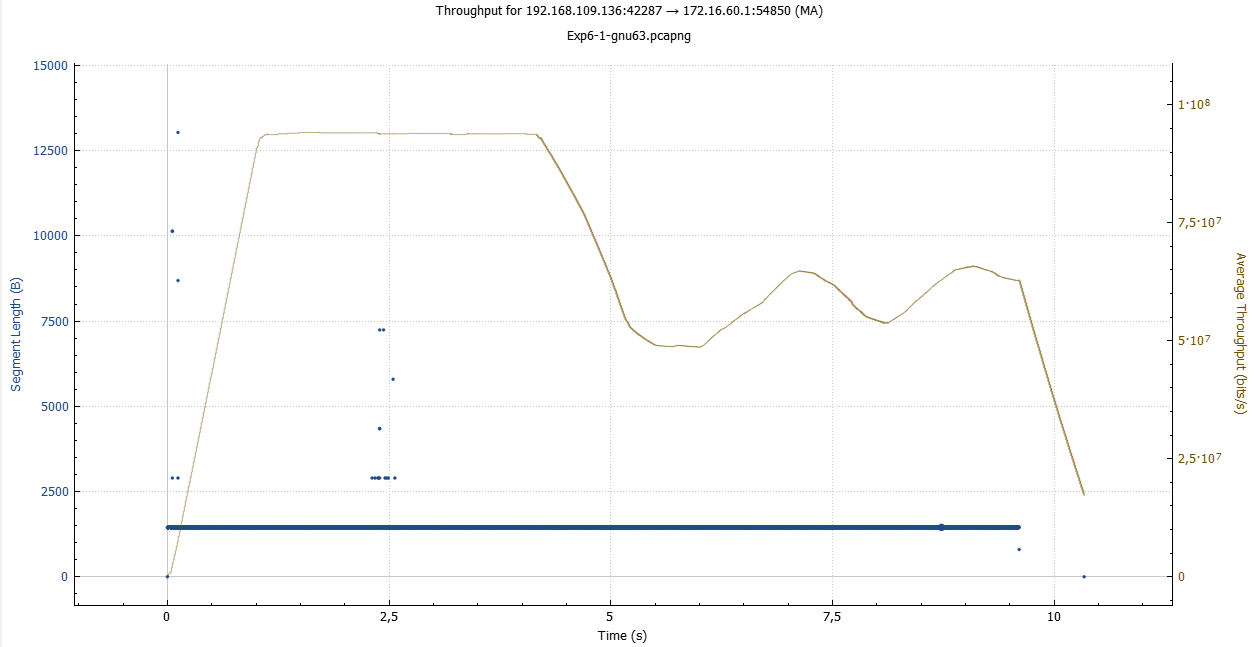
\includegraphics[scale=0.55]{exp6-step5-gnu63-graph.png}
\caption{Taxa de transferência no gnu63}
\end{figure}

\end{document}

